%%%%%%%%%%%%%%%%%%%%%%%%%%%%%%%%%%%%%%%%%
% Beamer Presentation
% LaTeX Template
% Version 1.0 (10/11/12)
%
% This template has been downloaded from:
% http://www.LaTeXTemplates.com
%
% License:
% CC BY-NC-SA 3.0 (http://creativecommons.org/licenses/by-nc-sa/3.0/)
%
%%%%%%%%%%%%%%%%%%%%%%%%%%%%%%%%%%%%%%%%%

%----------------------------------------------------------------------------------------
%	PACKAGES AND THEMES
%----------------------------------------------------------------------------------------

\documentclass{beamer}

\mode<presentation> {

% The Beamer class comes with a number of default slide themes
% which change the colors and layouts of slides. Below this is a list
% of all the themes, uncomment each in turn to see what they look like.

%\usetheme{default}
%\usetheme{AnnArbor}
%\usetheme{Antibes}
%\usetheme{Bergen}
%\usetheme{Berkeley}
%\usetheme{Berlin}
%\usetheme{Boadilla}
%\usetheme{CambridgeUS}
%\usetheme{Copenhagen}
%\usetheme{Darmstadt}
%\usetheme{Dresden}
%\usetheme{Frankfurt}
%\usetheme{Goettingen}
%\usetheme{Hannover}
%\usetheme{Ilmenau}
%\usetheme{JuanLesPins}
%\usetheme{Luebeck}
\usetheme{Madrid}
%\usetheme{Malmoe}
%\usetheme{Marburg}
%\usetheme{Montpellier}
%\usetheme{PaloAlto}
%\usetheme{Pittsburgh}
%\usetheme{Rochester}
%\usetheme{Singapore}
%\usetheme{Szeged}
%\usetheme{Warsaw}

% As well as themes, the Beamer class has a number of color themes
% for any slide theme. Uncomment each of these in turn to see how it
% changes the colors of your current slide theme.

%\usecolortheme{albatross}
%\usecolortheme{beaver}
%\usecolortheme{beetle}
%\usecolortheme{crane}
%\usecolortheme{dolphin}
%\usecolortheme{dove}
%\usecolortheme{fly}
%\usecolortheme{lily}
%\usecolortheme{orchid}
%\usecolortheme{rose}
%\usecolortheme{seagull}
%\usecolortheme{seahorse}
%\usecolortheme{whale}
%\usecolortheme{wolverine}

%\setbeamertemplate{footline} % To remove the footer line in all slides uncomment this line
%\setbeamertemplate{footline}[page number] % To replace the footer line in all slides with a simple slide count uncomment this line

%\setbeamertemplate{navigation symbols}{} % To remove the navigation symbols from the bottom of all slides uncomment this line
}
\usepackage{listings}
\usepackage{graphicx} % Allows including images
\usepackage{booktabs} % Allows the use of \toprule, \midrule and \bottomrule in tables

%----------------------------------------------------------------------------------------
%	TITLE PAGE
%----------------------------------------------------------------------------------------

\title[Lightning Network]{Bitcoin Transactions and Lightning Network} % The short title appears at the bottom of every slide, the full title is only on the title page

\author{Kwinten De Backer} % Your name

\date{\today} % Date, can be changed to a custom date

\begin{document}

\begin{frame}
\titlepage % Print the title page as the first slide
\end{frame}

\begin{frame}
\frametitle{Overview} % Table of contents slide, comment this block out to remove it
\tableofcontents % Throughout your presentation, if you choose to use \section{} and \subsection{} commands, these will automatically be printed on this slide as an overview of your presentation
\end{frame}

%----------------------------------------------------------------------------------------
%	PRESENTATION SLIDES
%----------------------------------------------------------------------------------------

%------------------------------------------------
\section{Bitcoin Transactions} % Sections can be created in order to organize your presentation into discrete blocks, all sections and subsections are automatically printed in the table of contents as an overview of the talk
%------------------------------------------------

\begin{frame}
\frametitle{General format of a Bitcoin transaction}
\begin{itemize}
\item Number of inputs
\item List of outputs
\item Number of outputs
\item List of outputs
\item LockTime
\end{itemize3}
\end{frame}
\begin{frame}
\frametitle{General format of a Bitcoin transaction}
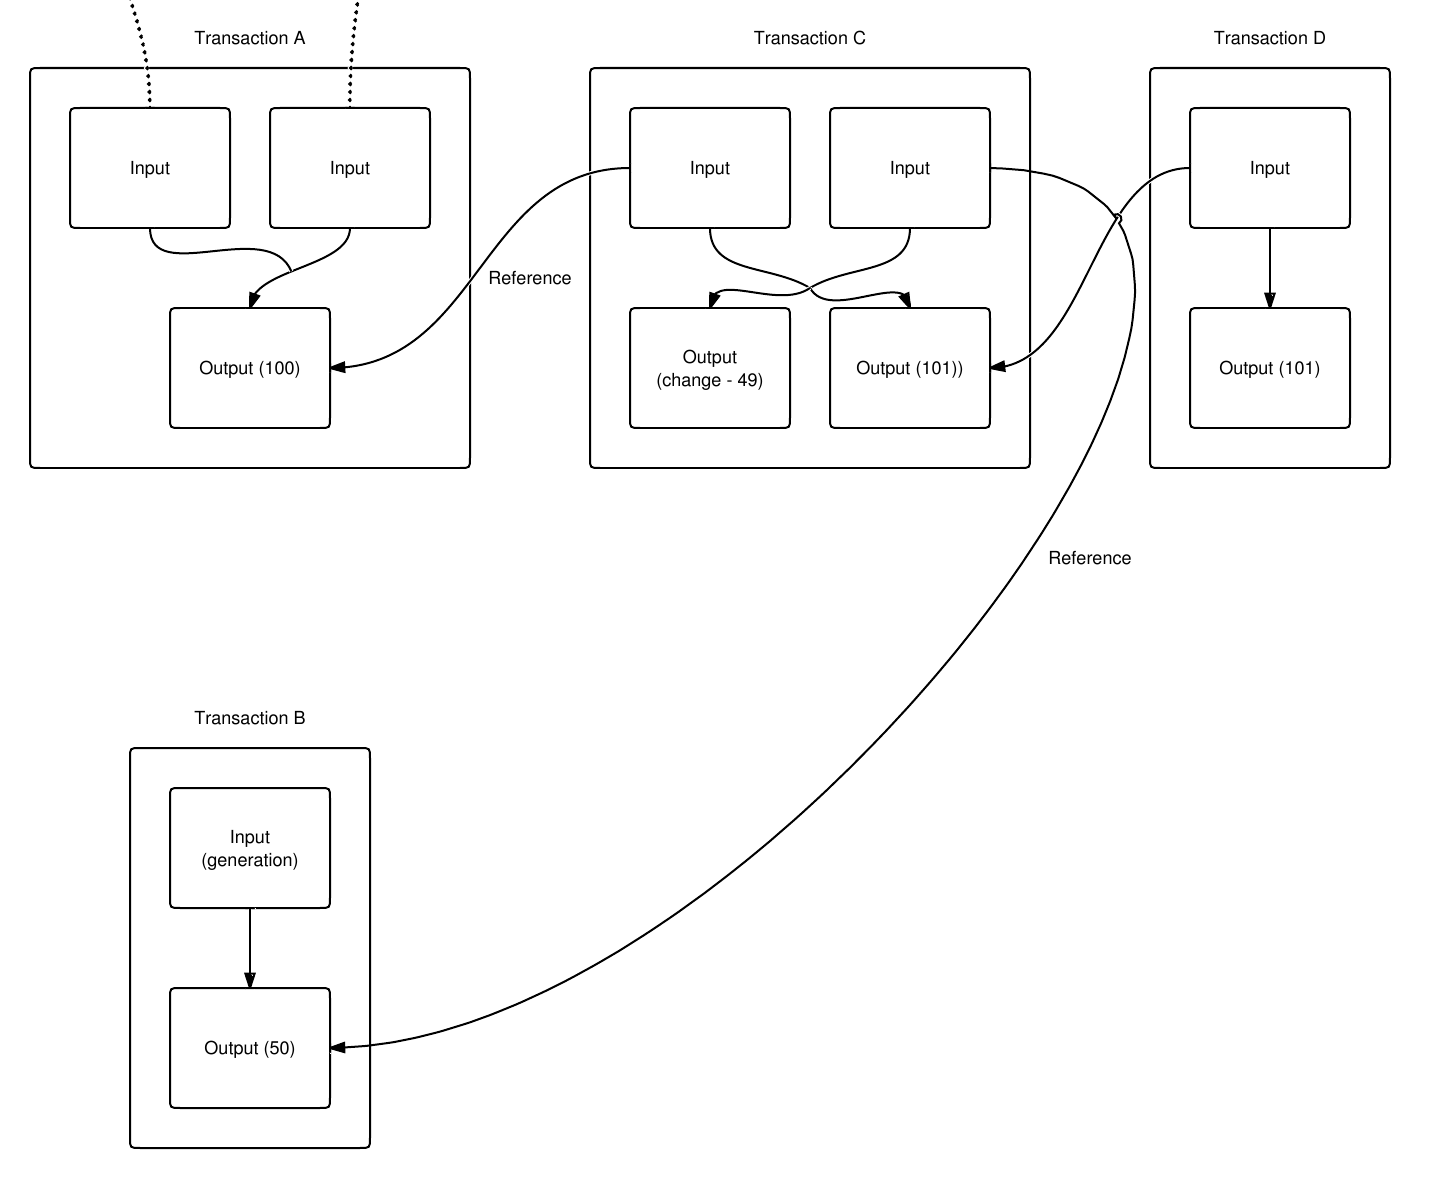
\includegraphics[scale=0.2]{images/transactions.png}
\end{frame}

%------------------------------------------------
\begin{frame}[fragile]
\textbf{Inputs} are references to \textbf{outputs} of previous transactions.

\textit{scriptSig} is the first part of the script
\frametitle{Inputs}
\begin{verbatim}Input:
Previous tx: f5d8ee39a430901c91a5917b9f2
dc19d6d1a0e9cea205b009ca73dd04470b9a6
Index: 0
scriptSig: 304502206e21798a42fae0e854281a
bd38bacd1aeed3ee3738d9e1446618c4571d10

90db022100e2ac980643b0b82c0
e88ffdfec6b64e3e6ba35e7ba5fdd7d5d6cc8d25c6b241501
\end{verbatim}
\end{frame}

\begin{frame}[fragile]
\frametitle{Outputs}
The total value of outputs must be less than the total value of the referenced outputs in the input part. 

\textit{scriptPubKey} is the second part of the script.
\begin{verbatim}
Output:
Value: 5000000000
scriptPubKey: OP_DUP OP_HASH160
 404371705fa9bd789a2fcd52
d2c580b65d35549d
OP EQUALVERIFY OP CHECKSIG
\end{verbatim}
\end{frame}

\begin{frame}
\frametitle{Verification}
Bitcoin uses a \textit{Forth}-like scripting language to check if a transaction is authorised. The parts in \textit{scriptSig} and \textit{scriptPubkey} are concatenated, pushed on a stack one by one and if the result is \textit{true}, the transaction is valid.
\end{frame}

\begin{frame}
\frametitle{What does it mean to own Bitcoin?}
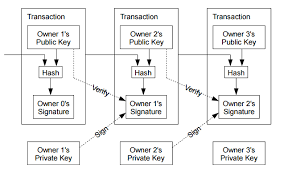
\includegraphics[scale=0.8]{images/chain.png}

\end{frame}

%------------------------------------------------

\begin{frame}
\frametitle{Pay to public key hash}
\begin{center}
\resizebox{350pt}{40pt}{
  \begin{tabular}{| l | c | r |}
    \hline
Stack&Script&Description \\ \hline
sig pubKey &OP DUP OP HASH160 pubKeyHash OPEQUALVERIFY OP CHECKSIG &	Constants are added to the stack. \\ \hline
sig pubKey pubKey &OP HASH160 pubKeyHash OP EQUALVERIFY OP CHECKSIG &	Top stack item is duplicated. \\ \hline
sig pubKey pubHashA &pubKeyHash OP EQUALVERIFY 
OP CHECKSIG&Top stack item is hashed. \\ \hline
sig pubKey pubHashA pubKeyHash&OP EQUALVERIFY OP CHECKSIG &	Constant added. \\ \hline
sig pubKey &OP CHECKSIG &Equality is checked between the top two stack items. \\ \hline
true&Empty.&Signature is checked for top two stack items. \\ \hline
  \end{tabular}
  }
\end{center}
\end{frame}

\begin{frame}[fragile]
\frametitle{Pay to script hash}
Created to move the responsability for supplying the conditions to 
redeem a transaction from the sender to the receiver. Makes funding a scripted transaction identical to funding a regular one.
\begin{verbatim}
scriptPubKey: OP_HASH160 <scriptHash> OP_EQUAL 
scriptSig: ..signatures... <serialized script>
\end{verbatim}
\end{frame}
\section{The double spending problem}
\begin{frame}
\frametitle{Mining (short)}
Transactions need to be included in a block by a miner to be considered valid, to protect against double spendings. The more blocks are added  on top of the block with the transaction, the more unlikely it is to be reversed. After 6 confirmations (1 hour), the transaction can safely be regarded as final.
\end{frame}
\section{Problems with scalability}
\begin{frame}
\frametitle{Transaction fees}
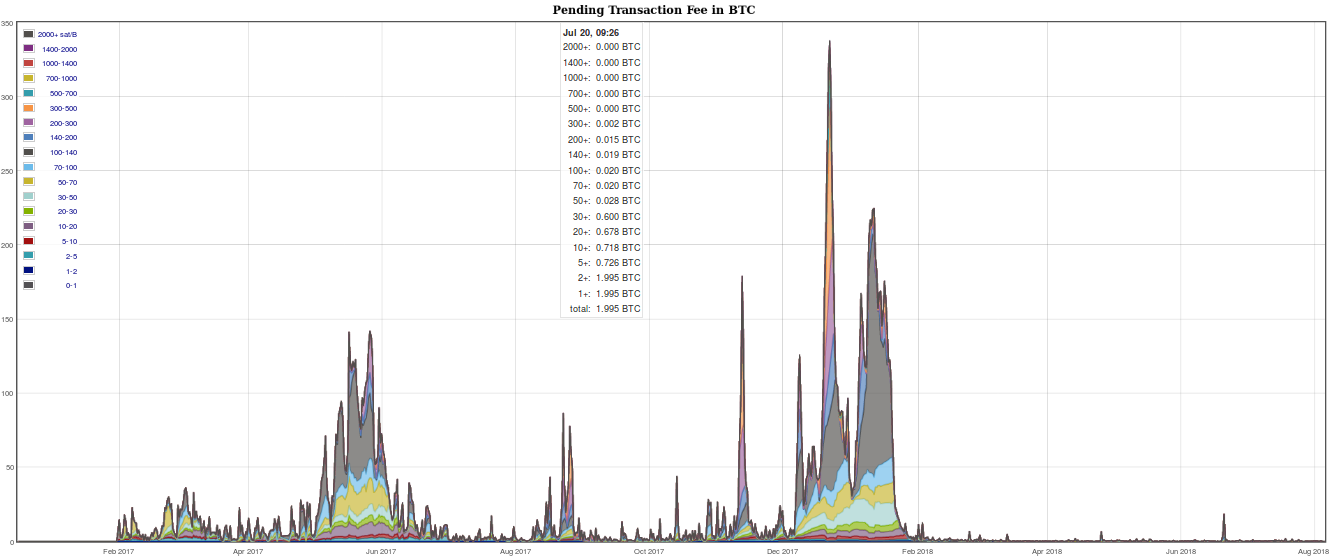
\includegraphics[scale=0.25]{images/fees.png}
\end{frame}
\begin{frame}
\frametitle{Blockspace and decentralization}
\textbf{All} of the properties Bitcoin has, it has because of it's decentralization. It is absolutely vital that the cost of running a node which validates all rules independently is kept as low as possible.
\begin{itemize}
\item Size of the Blockchain is already around 200 GB
\item Upload is around 200 GB/month, unmetered connection necessary.
\item Need to keep up with a new block every 10 minutes.
\end{itemize}
\end{frame}
\section{The Lightning Network}
\begin{frame}
\frametitle{Lightning on a conceptual level}

\end{frame}
\begin{frame}
\frametitle{Payment channels}

\end{frame}
\begin{frame}
\frametitle{Payment channel network (naive)}

\end{frame}
\begin{frame}
\frametitle{Payment channel network (better)}

\end{frame}
%------------------------------------------------

\begin{frame}
\frametitle{Lightning problems and solutions}

\end{frame}
\section{The real mindblowing stuff}
\begin{frame}
\frametitle{Cross chain atomic swaps}

\end{frame}
\begin{frame}
\frametitle{Submarine swaps}

\end{frame}

\begin{frame}
\frametitle{Oracles}

\end{frame}
\begin{frame}
\frametitle{Channel Factories}

\end{frame}
%------------------------------------------------

\begin{frame}
\frametitle{References}
\footnotesize{
\begin{thebibliography}{99} % Beamer does not support BibTeX so references must be inserted manually as below
\bibitem[Smith, 2012]{p1} John Smith (2012)
\newblock Title of the publication
\newblock \emph{Journal Name} 12(3), 45 -- 678.
\end{thebibliography}
}
\end{frame}

%------------------------------------------------

\begin{frame}
\Huge{\centerline{The End}}
\end{frame}

%----------------------------------------------------------------------------------------

\end{document} 
